\documentclass[10pt,utf8]{beamer}

\mode<presentation> {
  \usetheme{Madrid}
  \setbeamercovered{transparent}
}

\usepackage{palatino}
\usepackage{graphicx}
\usepackage{array}
\usepackage{color}
\usepackage{subfigure}
\usepackage{colortbl}
\usepackage{amsmath}
\usepackage{hyperref}
\usepackage{listings}
\usepackage{fancyvrb}

\setbeamertemplate{caption}{\raggedright\insertcaption\par} %turn off caption prefix ("Figure")

\definecolor{delim}{RGB}{20,105,176}
\definecolor{numb}{RGB}{106, 109, 32}
\definecolor{string}{rgb}{0.64,0.08,0.08}

\lstdefinestyle{java}{
	basicstyle          = \normalsize\ttfamily,
	language            = java,
	numbers             = left,
	numberstyle         = \small,
	stepnumber          = 1,
	numbersep           = 5pt,
	backgroundcolor     = \color{white},
	showspaces          = false,
	showstringspaces    = false,
	showtabs            = false,
	frame               = single,
	tabsize             = 2,
	captionpos          = b,
	breaklines          = true,
	breakatwhitespace   = false,
	morestring          = [b]",
	stringstyle         = \color{blue},
	keywordstyle        = \color{magenta},
	commentstyle        = \color{gray},
	identifierstyle     = \color{black},
	moredelim           = **[is][\bfseries]{`}{`},
	moredelim           = **[is][\color{magenta}]{$}{$}, 
	fancyvrb            = true,
}


\title{Virtual Threads in Debezium Engine}
\author{Vojtěch Juránek}
\institute[Red Hat]{Red Hat}
\date{November 18th 2025, Debezium F2F meeting, Prague}

\newenvironment{mylisting}
{\begin{list}{}{\setlength{\leftmargin}{1em}}\item\scriptsize\bfseries}
{\end{list}}

\newenvironment{mytinylisting}
{\begin{list}{}{\setlength{\leftmargin}{1em}}\item\tiny\bfseries}
{\end{list}}


\begin{document}

\begin{frame}
    \titlepage
\end{frame}

\begin{frame}
    \frametitle{Java threads}
    \begin{itemize}
        \item 1:1 mapping to OS threads.
        \item Memory heavy (MBs).
        \item Context switching is time consuming.
        \item Creation is expensive.
    \end{itemize}
\end{frame}

\begin{frame}
    \frametitle{Thread pooling}
    \begin{itemize}
        \item Doesn't solve memory overhead and context switching, just creating overhead.
        \item Issues with \texttt{ThreadLocal} and thread interrupts.
        \item Mitigate context switching $\rightarrow$ core-per-thread architecture.
    \end{itemize}
\end{frame}

\begin{frame}
    \frametitle{Asynchronous programming}
    \begin{itemize}
        \item Breaking tasks into smaller ones.
        \item Better CPU utilization, as blocking tasks (typically IO) are waiting in a queue instead blocking thread.
        \item Chaining usually via callbacks.
    \end{itemize}
\end{frame}

\begin{frame}
  \frametitle{Synchronous vs. asynchronous}
  \begin{columns}
        \column{0.6\textwidth}
            Synchronous:
            \begin{itemize}
                \item Simple to reason about it.
                \item Blocking.
                \item Less scalable.
            \end{itemize}
            
            \vspace{0.5cm}
            
            Asynchronous:
            \begin{itemize}
                \item Better scales.
                \item Harder to reason about it.
                \item ``Callback hell''.
                \item To get maximum benefit from it, all parts have to be asynchronous.
                \item Can be problematic to make it working with legacy synchronous code.
            \end{itemize}
            
        \column{0.4\textwidth}
            \begin{figure}
                \centering
                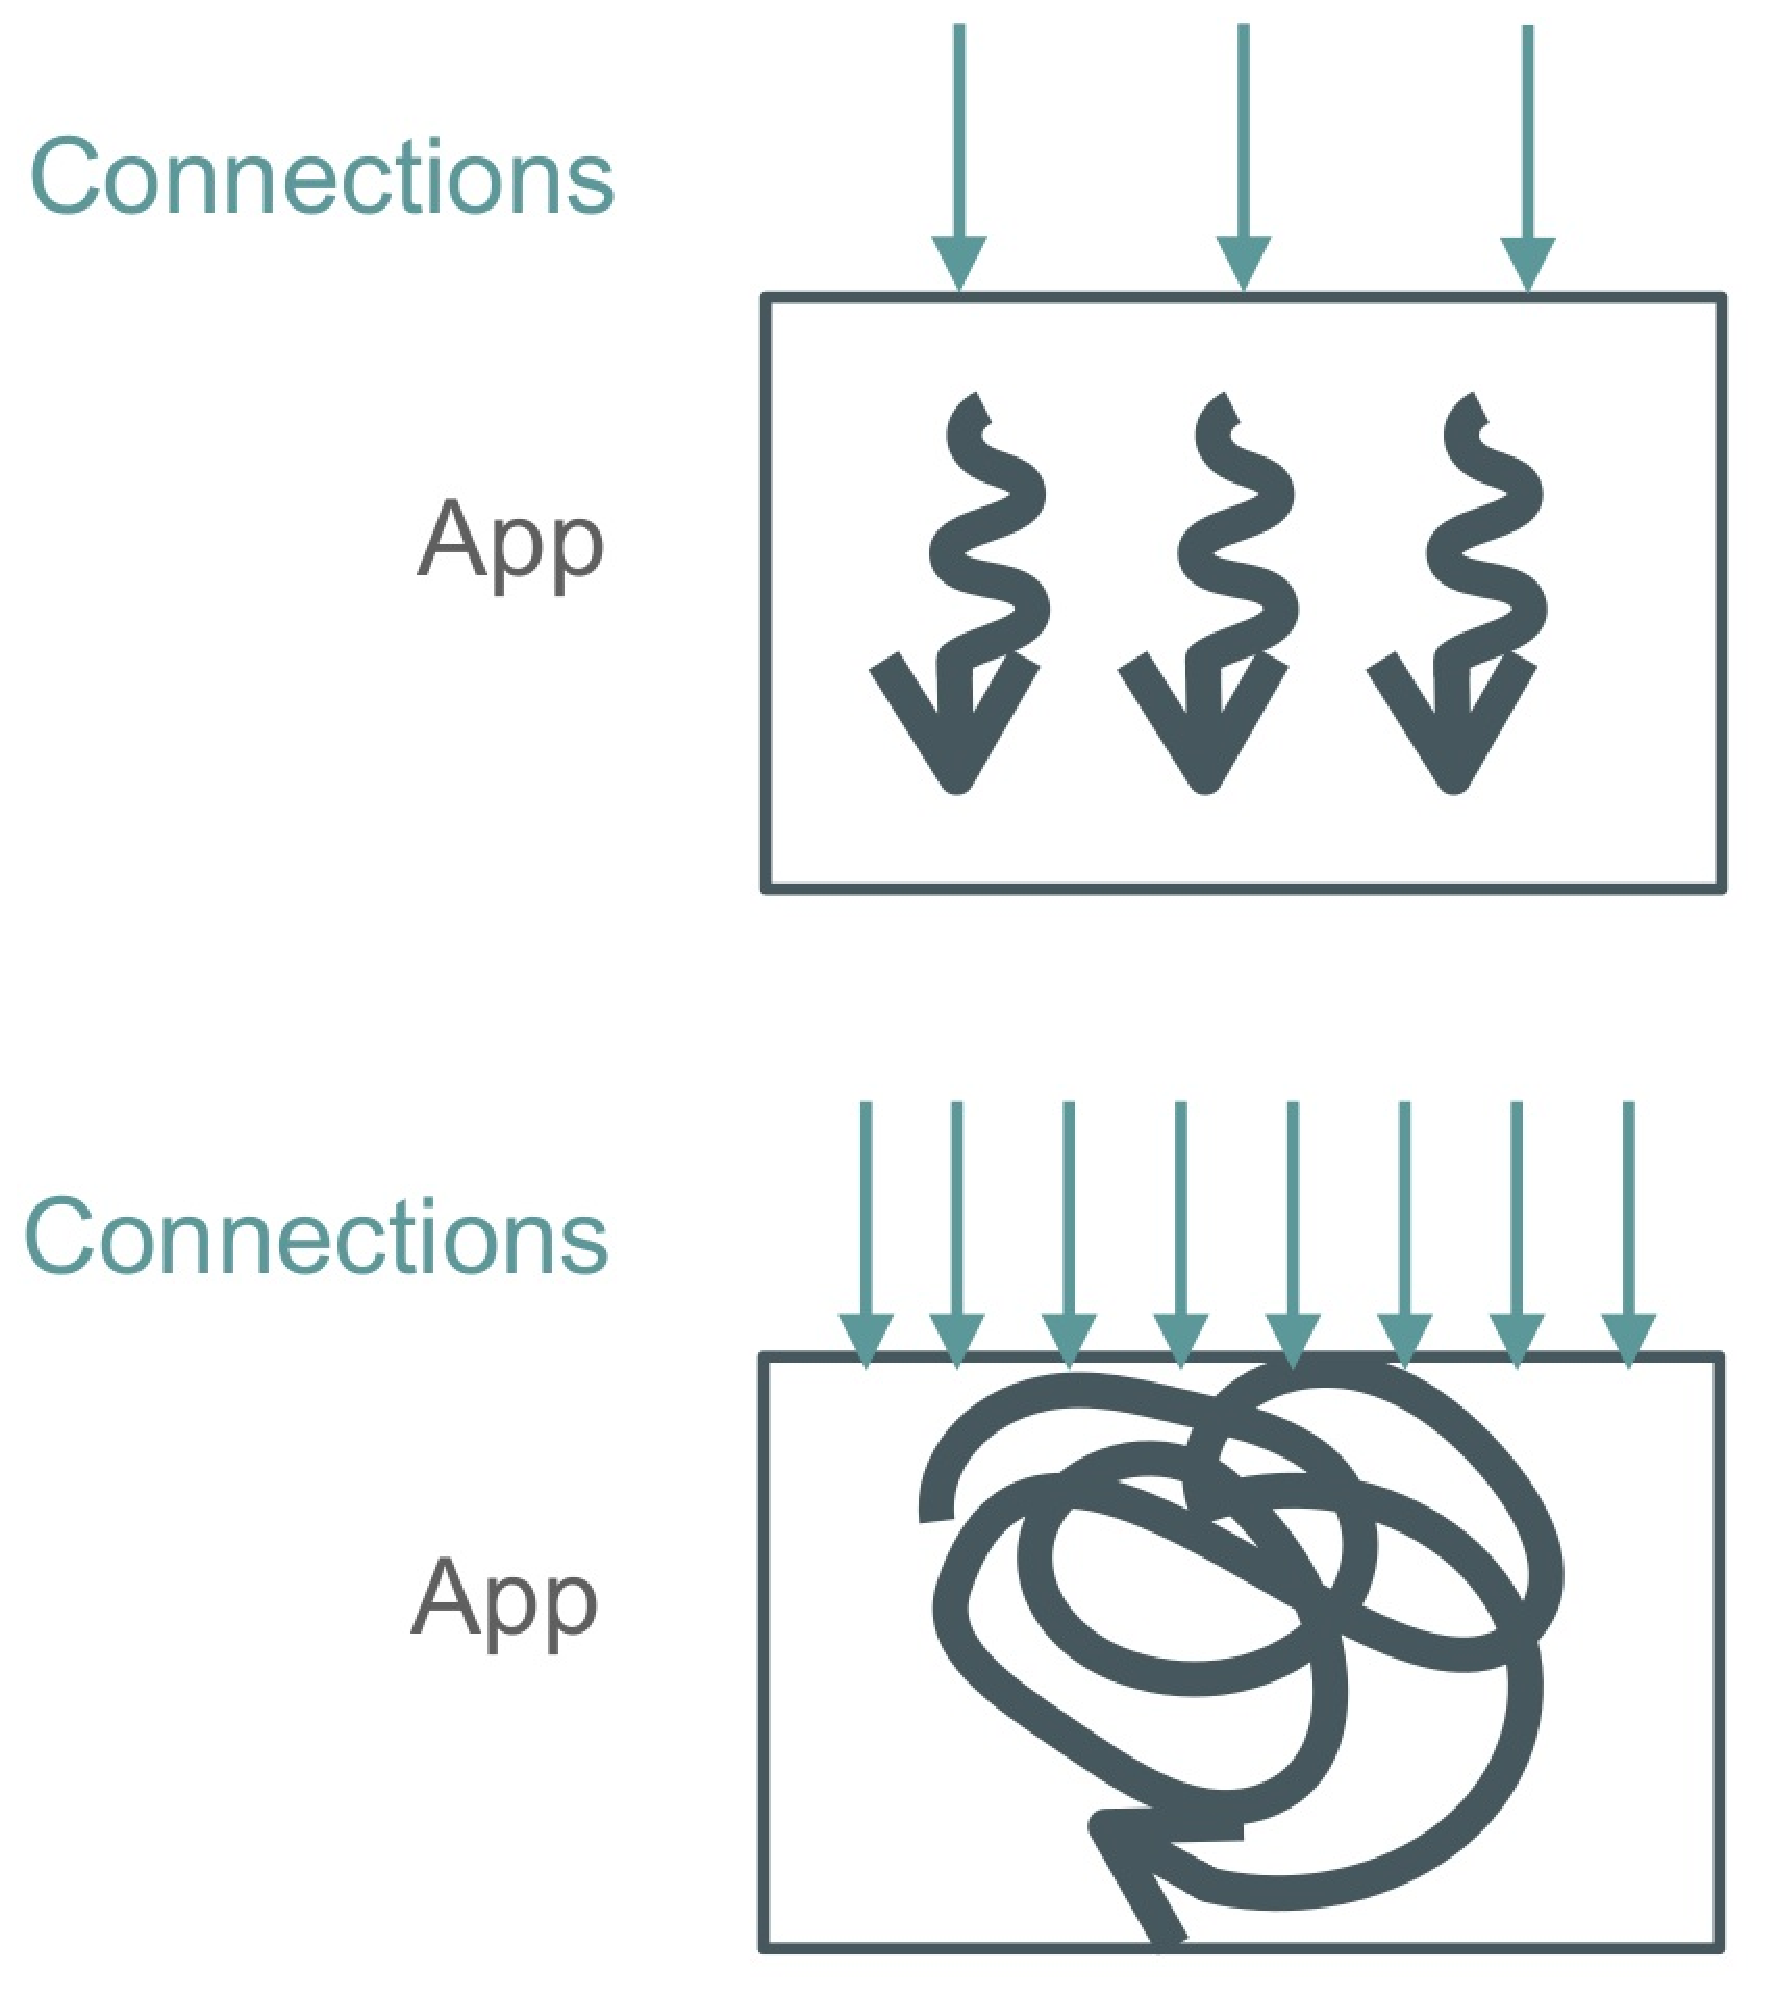
\includegraphics[height=5cm]{./img/sync_vs_async.eps}
                \caption{\tiny{Source: \url{http://cr.openjdk.java.net/~alanb/loom/Devoxx2018.pdf}}}
            \end{figure}
    \end{columns}
\end{frame}

\begin{frame}
    \frametitle{Java threads}
    What about having positives from both approaches:
    \begin{itemize}
        \item Code like synchronous code.
        \item Work like asynchronous code.
    \end{itemize}
    
    \begin{figure}
        \centering
        
\includegraphics[height=3cm]{./img/virt_threads.eps}
        \caption{\tiny{Source: \url{http://cr.openjdk.java.net/~alanb/loom/Devoxx2018.pdf}}}
    \end{figure}
\end{frame}

\begin{frame}
    \frametitle{Structured programming}
    \begin{figure}
        \centering
        Replacing \texttt{goto} with  \texttt{if-else}, \texttt{loop} statements and function calls in 60s:
        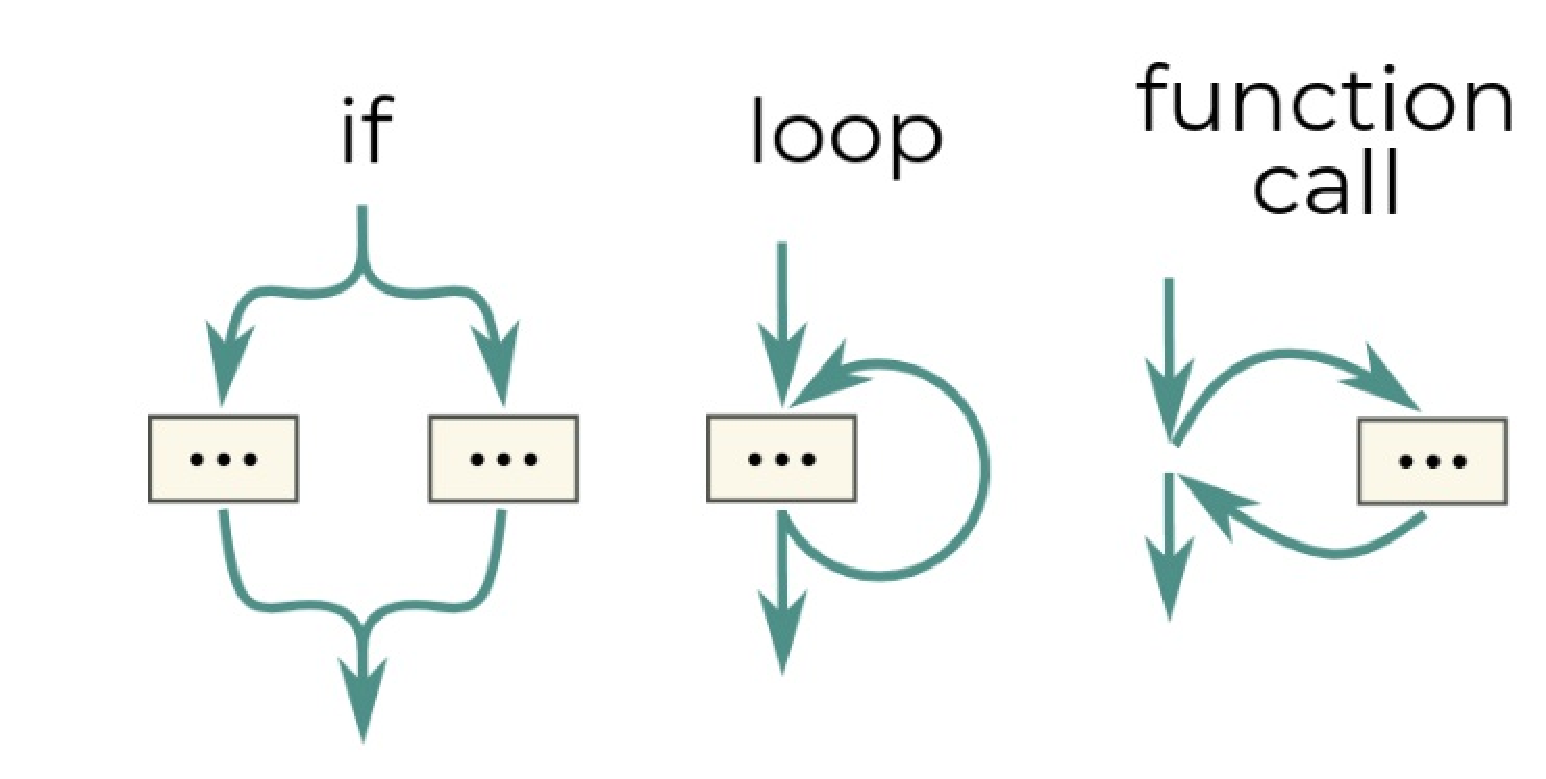
\includegraphics[height=5cm]{./img/structured.eps}
        \caption{\tiny{Source: \url{https://vorpus.org/blog/notes-on-structured-concurrency-or-go-statement-considered-harmful/}}}
    \end{figure}
\end{frame}

\begin{frame}
    \frametitle{Structured concurrency}
    \begin{itemize}
        \item Launching a task in a thread is like using \texttt{goto}.
        \item Structured concurrency is similar to using \texttt{if-else} and \texttt{loop} statements instead of \texttt{goto}.
    \end{itemize}

    \begin{figure}
        \centering
        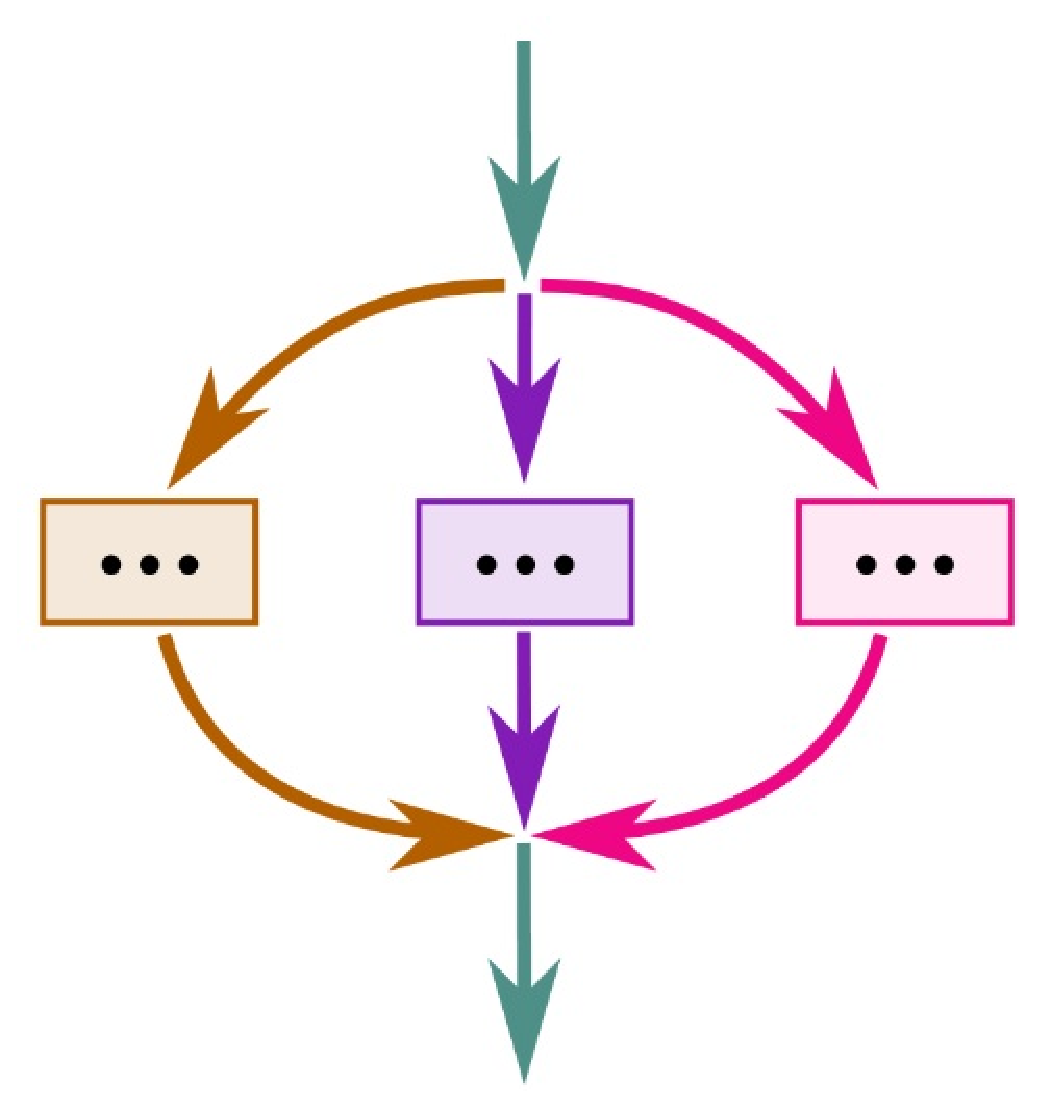
\includegraphics[height=5cm]{./img/structured_concurrency.eps}
        \caption{\tiny{Source: \url{https://vorpus.org/blog/notes-on-structured-concurrency-or-go-statement-considered-harmful/}}}
    \end{figure}
\end{frame}

\begin{frame}
    \frametitle{Java 25}
    \begin{itemize}
        \item Virtual threads (JEP 444) available and supported.
        \item Structured concurrency (JEP 505) is also available, but only as a preview feature (fifth preview).
    \end{itemize}
\end{frame}

\begin{frame}[fragile]
    \frametitle{First candidate for virtual threads - Asynchronous engine}
    \begin{lstlisting}[style=java]
final List<Future<R>> recordFutures = new ArrayList<>(records.size());
records.stream().forEachOrdered(r -> recordFutures.add(recordService.submit(new ProcessingCallables.TransformAndConvertRecord<R>(r, transformations, convertor))));

final List<R> convertedRecords = new ArrayList<>(recordFutures.size());
for (Future<R> f : recordFutures) {
    R record = f.get(); // we need the whole batch, eventually wait forever
    if (record != null) {
        convertedRecords.add(record);
    }
}
    \end{lstlisting}
\end{frame}

\begin{frame}
    \frametitle{Possible roadmap}
    \begin{itemize}
        \item Start replacing execution in threads by virtual threads in Debezium engine - pretty isolated and self-contained component.
        \item Measure, if there is any performance gain using JMH
        \item If there are no issue apply virtual threads also in rest of the Debezium.
        \item Once structured concurrency is available, apply start to use it as well.
    \end{itemize}
    
    \vspace{0.5cm}
    \centering \textbf{OR}
    \vspace{0.5cm}
    
    \begin{itemize}
        \item Wait until structured concurrency is supported and start with migration to virtual threads only after that.
        \item Wait for next LTS (Java 29 in September 2027)?
    \end{itemize}
\end{frame}


%%%%%%%%%%%%%%%%%%%%%%%%%%%%%%%%%%%%%%%%%%%%%%%%%%%%%%%%%%%%%%%%%%%%%%%%%%%%%%%%%%%%%%%%%%%%%%%%%
%%% BACKUP
%%%%%%%%%%%%%%%%%%%%%%%%%%%%%%%%%%%%%%%%%%%%%%%%%%%%%%%%%%%%%%%%%%%%%%%%%%%%%%%%%%%%%%%%%%%%%%%%%

% \begin{frame}
%     \centering
%     \huge{\textbf{Backup slides}}
% \end{frame}

\end{document}
